\documentclass{article}

\usepackage{graphicx}
\usepackage{amsmath}
\usepackage{fancyhdr}
\usepackage{listings}
\usepackage{xcolor}
\usepackage{textcomp}
\usepackage{float}
\usepackage[sorting=none]{biblatex}
\usepackage[margin=1in]{geometry}
\usepackage[font={small,it}]{caption}
\usepackage{placeins}
\usepackage{xepersian}

%\DeclareMathOperator*{\btie}{\bowtie}
\addbibresource{bibliography.bib}
\settextfont[Scale=1.2]{B-NAZANIN.TTF}
\setlatintextfont[Scale=1]{Times New Roman}
\renewcommand{\baselinestretch}{1.5}
\pagestyle{fancy}
\fancyhf{}
\rhead{تکلیف سوم درس پایگاه داده‌ها 1}
\lhead{\thepage}
\rfoot{علیرضا ابره فروش}
\lfoot{9816603}
\renewcommand{\headrulewidth}{1pt}
\renewcommand{\footrulewidth}{1pt}
%%%%%%%%%%
\lstset
{
    language=[latex]tex,
    basicstyle=\ttfamily,
    commentstyle=\color{black},
    columns=fullflexible,
    keepspaces=true,
    upquote=true,
    showstringspaces=false,
    morestring=[s]\\\%,
    stringstyle=\color{black},
}
%%%%%%%%%%

\begin{document}
\begin{titlepage}
\begin{center}

\includegraphics[width=0.4\textwidth]{figures/IUT Logo.png}\\
        
\LARGE
\textbf{دانشگاه صنعتی اصفهان}\\
\textbf{دانشکده مهندسی برق و کامپیوتر}\\
        
\vfill
        
\huge
\textbf{عنوان: تکلیف چهارم درس ریزپردازنده}\\
        
\vfill
        
\LARGE
\textbf{نام و نام خانوادگی: علیرضا ابره فروش}\\
\textbf{شماره دانشجویی: 9816603}\\
\textbf{نیم\,سال تحصیلی: پاییز 1400}\\
\textbf{مدرّس: دکتر عارف کریمی افشار}\\
\end{center}
\end{titlepage}


%\tableofcontents
\newpage


\section{1}
\subsection{\lr{a}}
نام دانشکده‌هایی را برمی‌گرداند که بودجه(مجموع حقوق اساتید)ی آن‌ها از میانگین بودجه‌ی همه دانشکده‌ها بیشتر یا مساوی است.
\begin{figure}[H]
    \centering
    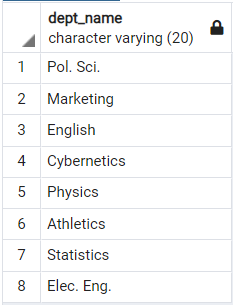
\includegraphics[width=0.3\textwidth]{figures/1-a.png}
    \caption
	{
\lr{1-a}
	}
    \label{fig:fig1}
\end{figure}

\subsection{\lr{b}}
نام اساتیدی را بر‌می‌گرداند که تعداد درس‌های ارائه شده توسط آن‌ها در سال 2003 از میانگین تعداد درس‌های ارائه شده در آن سال بیشتر است.
\begin{figure}[H]
    \centering
    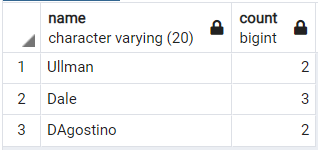
\includegraphics[width=0.3\textwidth]{figures/1-b.png}
    \caption
	{
\lr{1-b}
	}
    \label{fig:fig1}
\end{figure}


\section{2}
\subsection{\lr{a}}
\begin{figure}[H]
    \centering
    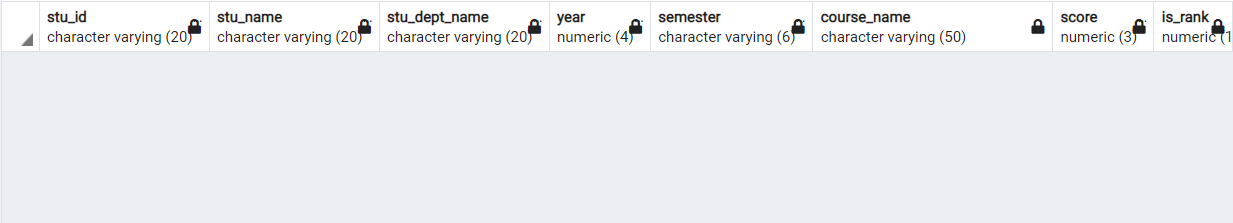
\includegraphics[width=0.8\textwidth]{figures/2-a.png}
    \caption
	{
\lr{2-a}
	}
    \label{fig:fig1}
\end{figure}

\subsection{\lr{b}}
\begin{figure}[H]
    \centering
    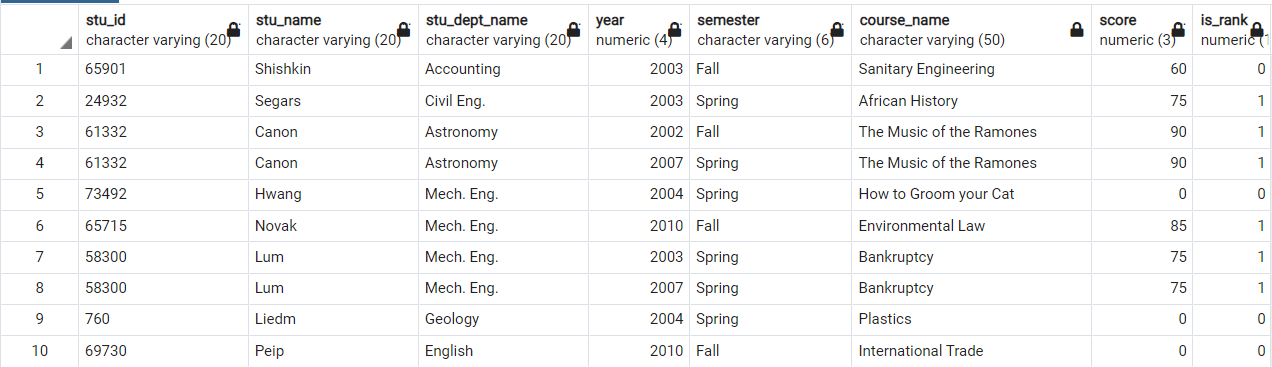
\includegraphics[width=0.8\textwidth]{figures/2-b.png}
    \caption
	{
\lr{2-b}
	}
    \label{fig:fig1}
\end{figure}

\subsection{\lr{c}}
\begin{figure}[H]
    \centering
    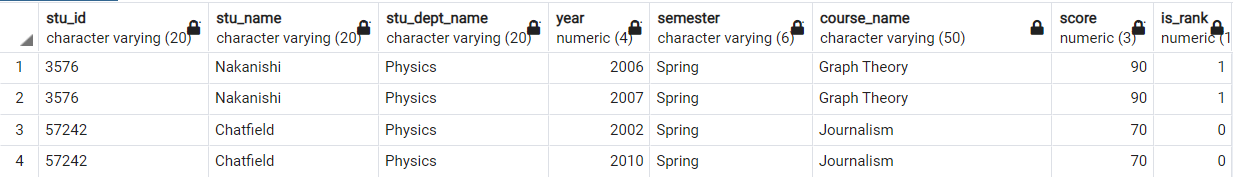
\includegraphics[width=0.8\textwidth]{figures/2-c-before.png}
    \caption
	{
\lr{2-c(before running query)}
	}
    \label{fig:fig1}
\end{figure}
\begin{figure}[H]
    \centering
    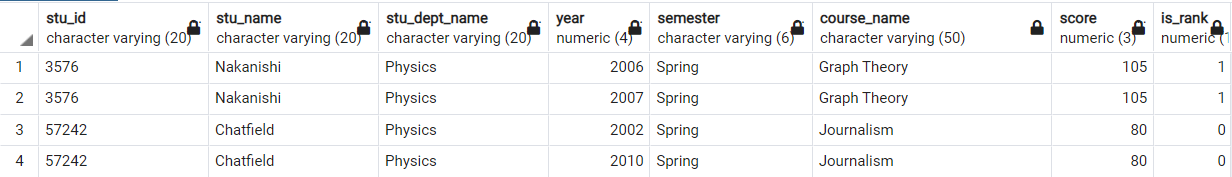
\includegraphics[width=0.8\textwidth]{figures/2-c-after.png}
    \caption
	{
\lr{2-c(after running query)}
	}
    \label{fig:fig1}
\end{figure}

\subsection{\lr{d}}
\begin{figure}[H]
    \centering
    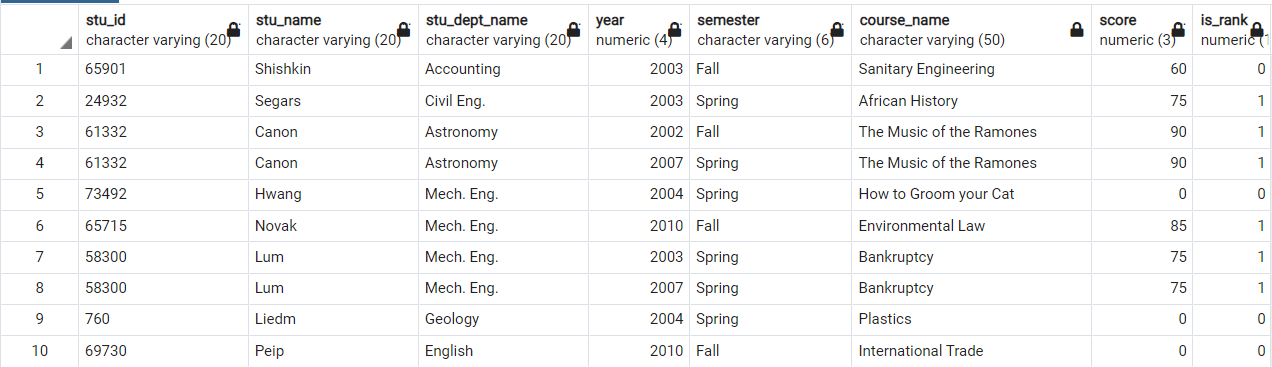
\includegraphics[width=0.8\textwidth]{figures/2-b.png}
    \caption
	{
\lr{2-d}
	}
    \label{fig:fig1}
\end{figure}


\section{3}
\begin{table}[H]
    \centering
    \begin{tabular}{|c|c|c|}
    \hline
    \textbf{بیشترین تعداد خروجی حاصل} & \textbf{کمترین تعداد خروجی حاصل} & \textbf{}\\
    \hline
    100 & 100 & \lr{users INNER JOIN numbers}\\
    \hline
    199 & 100 & \lr{users LEFT OUTER JOIN numbers}\\
    \hline
    100 & 100 & \lr{users RIGHT OUTER JOIN numbers}\\
    \hline
    199 & 100 & \lr{users FULL OUTER JOIN numbers}\\
    \hline

    \end{tabular}
    \caption{جدول شماره 1}
    \label{tab:tab1}
\end{table}

\section{4}
\subsection{\lr{a}}
\begin{figure}[H]
    \centering
    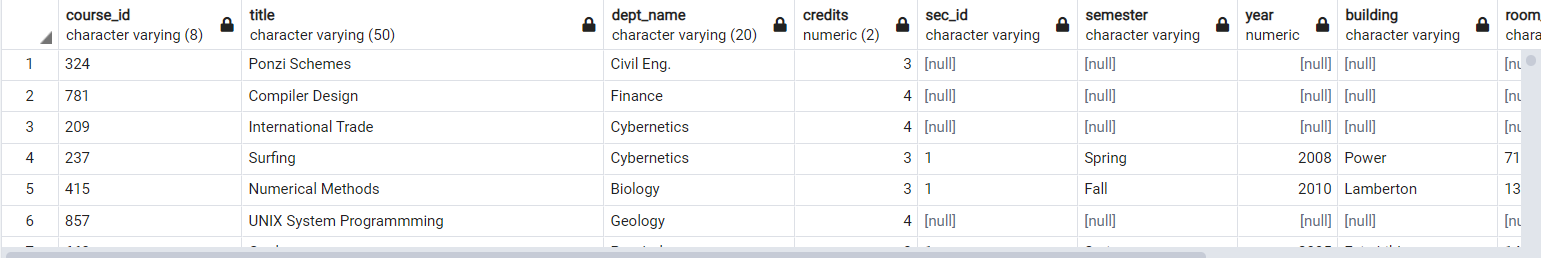
\includegraphics[width=0.8\textwidth]{figures/4-a.png}
    \caption
	{
\lr{4-a}
	}
    \label{fig:fig1}
\end{figure}

\subsection{\lr{b}}
\begin{figure}[H]
    \centering
    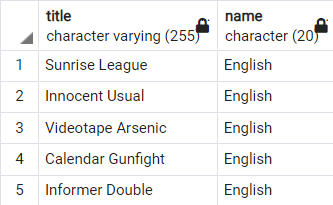
\includegraphics[width=0.8\textwidth]{figures/4-b.png}
    \caption
	{
\lr{4-b}
	}
    \label{fig:fig1}
\end{figure}

\subsection{\lr{c}}
\begin{figure}[H]
    \centering
    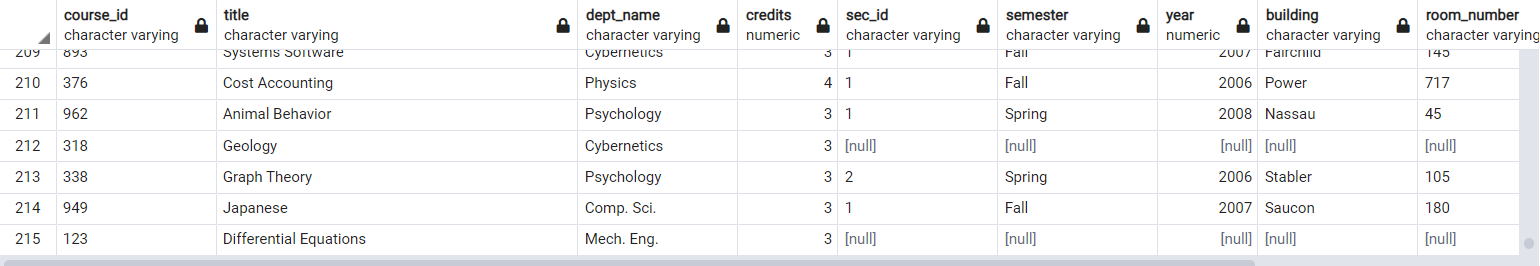
\includegraphics[width=0.8\textwidth]{figures/4-c.png}
    \caption
	{
\lr{4-c}
	}
    \label{fig:fig1}
\end{figure}

\section{5}
\subsection{\lr{a}}
\begin{figure}[H]
    \centering
    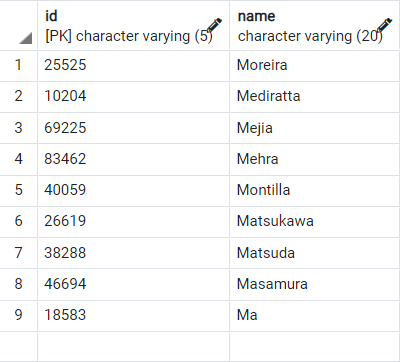
\includegraphics[width=0.8\textwidth]{figures/5-a.png}
    \caption
	{
\lr{5-a}
	}
    \label{fig:fig1}
\end{figure}

\subsection{\lr{b}}
\begin{figure}[H]
    \centering
    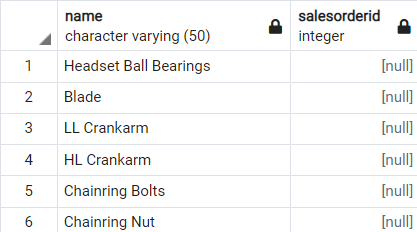
\includegraphics[width=0.8\textwidth]{figures/5-b.png}
    \caption
	{
\lr{5-b}
	}
    \label{fig:fig1}
\end{figure}

\subsection{\lr{c}}
\begin{figure}[H]
    \centering
    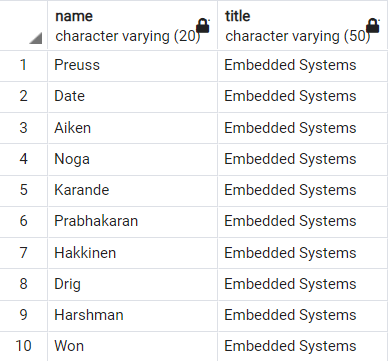
\includegraphics[width=0.8\textwidth]{figures/5-c.png}
    \caption
	{
\lr{5-c}
	}
    \label{fig:fig1}
\end{figure}

\subsection{\lr{c}}
\begin{figure}[H]
    \centering
    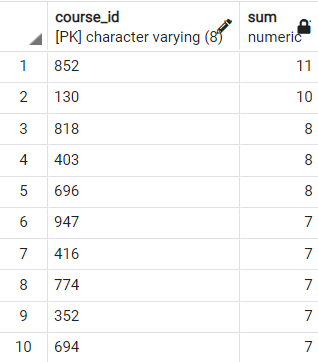
\includegraphics[width=0.8\textwidth]{figures/5-d.png}
    \caption
	{
\lr{5-d}
	}
    \label{fig:fig1}
\end{figure}

\section{6}
\begin{figure}[H]
    \centering
    
\includegraphics[width=0.8\textwidth]{figures/6.png}
    \caption
	{
\lr{6}
	}
    \label{fig:fig1}
\end{figure}

\section{7}
\begin{figure}[H]
    \centering
    
\includegraphics[width=0.8\textwidth]{figures/7.png}
    \caption
	{
\lr{7}
	}
    \label{fig:fig1}
\end{figure}

\section{8}
\begin{figure}[H]
    \centering
    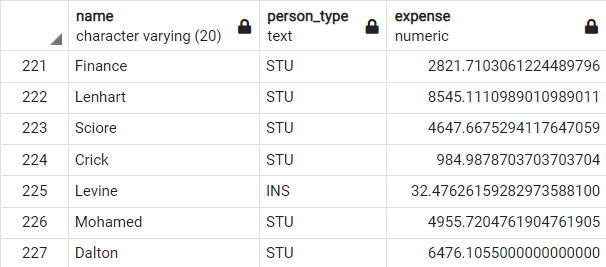
\includegraphics[width=0.8\textwidth]{figures/8.png}
    \caption
	{
\lr{8}
	}
    \label{fig:fig1}
\end{figure}
%------------------------------------------------------------------------------------------


\section*{منابع}
\renewcommand{\section}[2]{}%
\begin{thebibliography}{99} % assumes less than 100 references
%چنانچه مرجع فارسی نیز داشته باشید باید دستور فوق را فعال کنید و مراجع فارسی خود را بعد از این دستور وارد کنید


\begin{LTRitems}

\resetlatinfont

\bibitem{b1} https://searchoracle.techtarget.com/answer/LEFT-OUTER-JOIN-without-using-LEFT-OUTER-JOIN
\end{LTRitems}

\end{thebibliography}


\end{document}
